\documentclass[12pt]{article}
\usepackage[czech]{babel}
\usepackage[utf8]{inputenc}
\usepackage[plainpages=false,pdfpagelabels,unicode]{hyperref}
\usepackage[pdftex]{graphicx}
\usepackage[margin=2cm, includefoot]{geometry}

\begin{document}

\title{Otázky ke státnícím -- plazma 5 \\
Technologie vytváření tenkých vrstev, modifikace povrchů, diagnostika}
\maketitle

\section{Metody depozice tenkých vrstev}
Tak tady je toho hodně, některé jsou více chemické, třeba elektrolytické nanášení, oxidace, tepelná oxidace, depozice z plynné fáze (CVD) a adsorpce. Z takových více fyzikálních metod zmíním základní tři: napařování, PECVD a naprašování. 

\subsection{Napařování}
Velmi jednoduchý proces, požadovaný materiál se odpaří a pak kondenzuje na substrát. Praktický příklad viz protokol z vakuového praktika, kde jsme napařovali tuším stříbro na sklo. Celý proces probíhá za vysokého vakua, čím lepší vakuum tím líp. Je to výborný proces pro napařování tenkých kovových vrstev. Nevýhodou je vysoká teplota, může docházet k poškození substrátu, a také třeba k pnutí (když má substrát a vrstva rozdílnout teplotní roztažnost). Také to třeba nefunguje dobře na slitiny, protože různé prvky se vypařují při různých teplotách. Pro zahřívání se používá buď ohmický ohřev a nebo ohřev elektronovým svazkem. Dopadající atomy mají Maxwellovo rozložení rychlosti.

\subsection{PECVD}
Obdoba principu chemické depozice z plynné fáze. Používá se neizotermické plazma, tj. rychlé elektrony a pomalé ionty. Ionty a neutrální plyn mají většinou pokojovou teplotu. Reakcemi energetických elektronů s neutrály dochází k ionizaci, disociaci molekul a polymerů atd... Případně může naopak v plazmě docházet k plazmové polymerizaci --růstu polymerů z monomerů. To vše za nízkých teplot! Kromě reakcí v plazmatu je dále důležité chování částic ve stěnové vrstvě. Tam je stejnosměrné předpětí, které vzniká jednak klasickým rozdílem mezí potenciálem plazmatu a stěnovým potenciálem, případně podle typu výboje i dalšími jevy. Regulací stejnosměrného předpětí mezi plazmatem a substrátem můžeme regulovat vlastnosti (především energii) dopadajících části a vytvářet široké spektrum vrstev.

Pro depozice se většinou používá RF napětí, protože tak můžeme deponovat i dielektrické vrstvy. Pokud bychom používali stejnosměrné, docházelo by k napíjení vrstev a úbytku stejnosměrného předpětí. Dopadající ionty mají většinou poměrně úzké rozložení rychlostí. Jak moc je rozšířené záleží jednak na tlaku (jak moc dochází ke srážkám ve stěnové vrstvě) a v případě střídavého výboje také na frekvenci. Pokud je čas průletu iontu stěnovou vrstvou výrazně menší než perioda napětí, dochází ke vzniku dvou výrazných píků v rozložení rychlosti (viz slidy z plazmatu 2).

\subsection{Naprašování}
Princip naprašování spočívá v bombardování terče (typicky katody) vysokoenergetickými ionty, vyražené atomy terče se pak deponují na substrát. K vytvoření svazku iontů lze použít více metod, nejvíce používané je magnetronové naprašování.

\begin{figure}
\centering
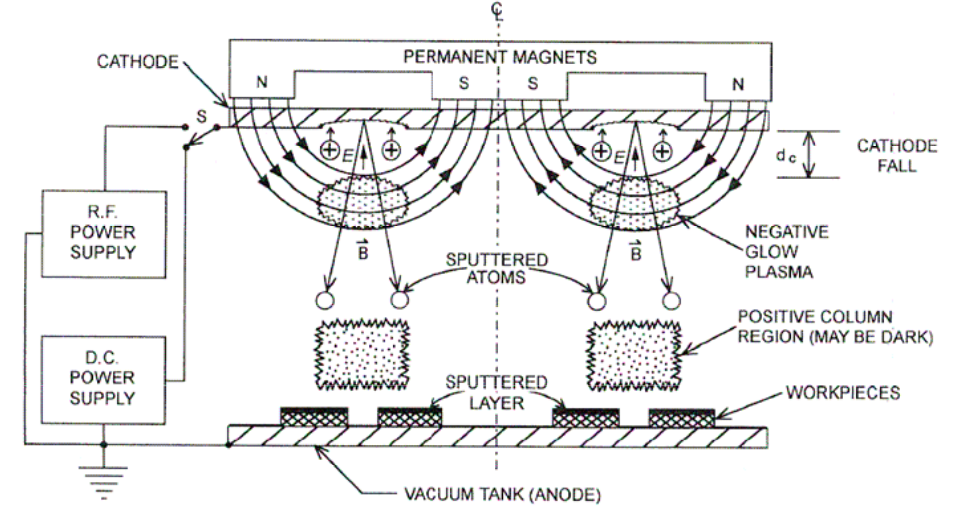
\includegraphics{magnetron2.png}
\caption{Schéma magnetronu}
\label{magnetron}
\end{figure}

Schéma magnetronu je na obrázku \ref{magnetron}. V magnetronu hoří anomální doutnavý výboj (ten je typický tím, že v něm není potenciál rozložen rovnoměrně ale u katody je tzv. katodový spád), může být napájen RF nebo DC napětím. Opět platí, že čím větší vakuum, tím lépe. Vyražené atomy difundují na substrát, nicméně při moc vysokém vakuu může dojít k vyhasnutí výboje. Magnetické pole slouží k prodloužení dráhy elektronů, zvýšení srážkové frekvence a také vzniká efekt magnetického zrcadla. Toto vše vede k větší ionizaci a umožňuje výboji hořet i při nižších tlacích. Elektrony jsou především koncentrovány v oblasti záporného (katodového) světla. Další možné uspořádání je třeba koplanární magnetron, kdy anoda není naproti katody ale vedle. Ionty jsou urychlovány v oblasti katodového spádu. Více informací třeba v prezentaci z Plasmy 2 \url{https://is.muni.cz/auth/el/1431/jaro2012/F8242/um/Lekcia_07_2012.pdf}


\section{Měření parametrů tenkých vrstev (tloušťka, tvrdost, adheze, ...) }
\subsection{Tloušťka}
\subsubsection{Kalotest}
Velmi jednoduché měření tloušťky vrstev. Do vrstvy vybrousíme kulový vrchlík koulí o přesně definovaném průměru, ten pak změříme pod mikroskopem a z velikostí průmětů do substrátu a do vrstvy se vypočítá tloušťka vrstvy.
\subsubsection{Vážení vrstvy}
Zvážíme substrát bez vrstvy, pak s vrstvou, pokud známe hustotu, můžeme určit tloušťku, případně pokud tloušťku určíme jinak, jde určit hustota. Nevýhodou je potřeba velmi přesných vah a měření může být výrazně ovlivněno třeba adsorpcí na vrstvě.
\subsubsection{Změna frekvence vibrací krystalu}
Vzpomeň na vakuové praktikum, kde jsme to používali k určení tloušťky vrstvy při napařování. Vrstva se napařuje na krystal, měří se změna vlastní frekvence.
\subsubsection{Interference}
viz optika dále
\subsubsection{Elektrické metody}
Měři se změna el. odporu, kapacitance atd.


\subsection{Tvrdost}
\subsubsection{Indentační test}
Vrstvy napichujeme přesně definovaným hrotem (většinou troj nebo čtyřstěnná pyramida) a měříme buď celkovou velikost vpichu po indentaci, případně závislost hloubky indentace na síle vpichu (to se měří tam i zpět a lze tedy rozlišit elastické a neelastické deformace). Tenké vrstvy se typicky měří tzv nanoindentory, kde síla vpichu je velmi malá (řádově 10--100\,$\mu$N), abychom zamezili vlivu substrátu.

\subsection{Adheze}
\subsubsection{Scratch test}
Měření adheze, hrotem škrábeme po povrchu, síla se lineárně zvětšuje, zajímá nás především v jaké vzdálenosti od začátku dojde k delaminaci vrstv

\subsection{Povrchová energie}
\subsubsection{Měření kontaktního úhlu}
Nebudu rozepisovat, viz protokol ze speciálního praktika. 


\begin{figure}[ht]
\begin{minipage}[b]{0.45\linewidth}
\centering
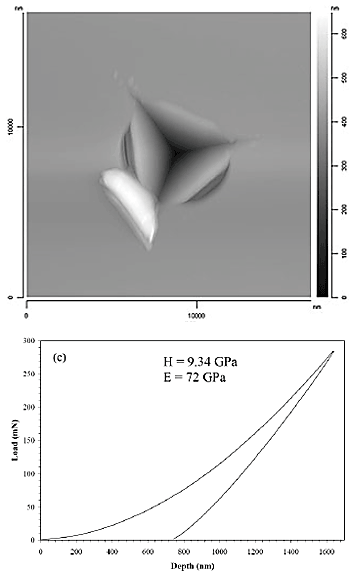
\includegraphics[width=\textwidth]{berkovitz.png}
\caption{Indentační test}
\label{fig:figure1}
\end{minipage}
\hspace{0.5cm}
\begin{minipage}[b]{0.45\linewidth}
\centering
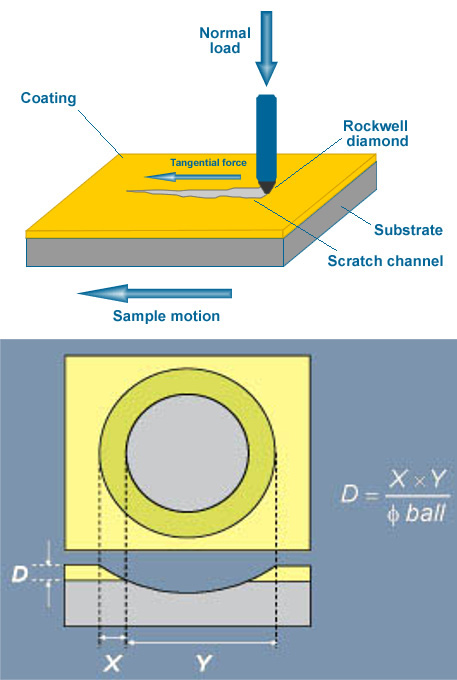
\includegraphics[width=\textwidth]{scratchandcalo.jpg}
\caption{Scratch test (nahoře) a kalotest (dole)}
\label{fig:figure2}
\end{minipage}
\end{figure}

\subsection{Optika}
Optickými metodami se dá měřit velmi široké spektrum vlastností látek, přes optické veličiny jako komplexní index lomu a tloušťka vrstvy, přes parametry elektronové struktury, chemické složení hustotu atd. Optika nelze ale použít vždy, je velmi citlivá na různé defekty jako třeba nehomogenita, neuniformita, povrchová drsnost, drsnost rozhraní vrstvy -- substrátu, nečistoty atd... 

Důležitý je mít dobrý disperzní model (závislost indexu lomu, případně komplexního indexu lomu na vlnové délce). Příklad třeba Cauchyho formule, nebo Lotrentzův oscilátor, případně modely kde parametrizujeme přímo hustotu stavů. Tohle ale už jde hodně do pevných látek, takže asi moc nezmiňovat.

Teď trochu opakování z Kmitů vln a optiky (optiku mám rozepsanou podrobněji, protože je to moje specializace, ale klidně to lze ignorovat...)

Na rozhraní dvou prostředí s rozdílnými indexy lomu se světlo láme dle Snellova zákona
\begin{equation}
\hat{n}_0 \sin\hat{\theta}_0 = \hat{n}_1 \sin\hat{\theta}_1 \mathrm{.}
\end{equation}
Fresnelovy koeficienty na~rozhraní jsou pro s polarizovanou vlnu: 
\begin{equation}
\hat{r}_\mathrm{s} = \frac{ \hat{n}_0 \cos \hat{\theta}_0 - \hat{n}_1 \cos \hat{\theta}_1}{ \hat{n}_0 \cos \hat{\theta}_0 + \hat{n}_1 \cos \hat{\theta}_1}  \mathrm{,}
\end{equation}
pro p polarizovanou vlnu: 
\begin{equation}
\hat{r}_\mathrm{p} = \frac{ \hat{n}_0 \cos \hat{\theta}_1 - \hat{n}_1 \cos \hat{\theta}_0}{ \hat{n}_0 \cos \hat{\theta}_1 + \hat{n}_1 \cos \hat{\theta}_0}  \mathrm{.}
\end{equation}
Indexy lomu i úhly jsou obecně komplexní ($\hat{n}_i = n_i + \mathrm{i} \kappa_i$).

\begin{figure}
  \centering
  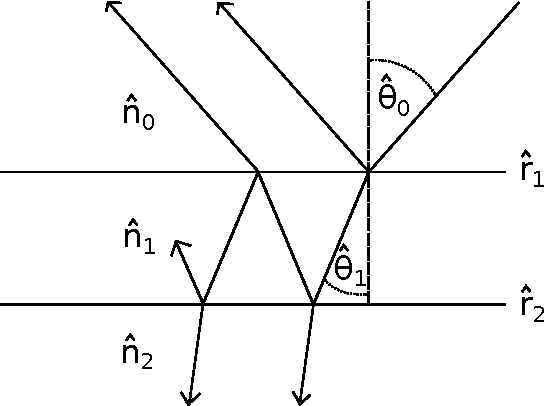
\includegraphics[width=80mm]{schema.pdf}
  \caption{Schéma rozhraní vzduch--vrstva--substrát}
  \label{schema}
\end{figure}

\subsubsection{Odrazivost}
Odrazivost R je definována jako průměr odrazivostí pro s a~p polarizované světlo 
%
\begin{equation} R = \frac{1}{2}(R_\mathrm{s} + R_\mathrm{p})\, \mathrm{,}\end{equation}
%
kde $R_\mathrm{s} = |\hat{r}_\mathrm{s}|^2$, $R_\mathrm{p} = |\hat{r}_\mathrm{p}|^2$.
Pro celkovou odrazivost systému vzduch--vrstva--substrát (obrázek \ref{schema}) platí 
\begin{equation} R = \left|\frac{\hat{r}_1 + \hat{r}_2 \mathrm{e}^{\mathrm{i}\hat{\alpha}} }{1 + \hat{r}_1 \hat{r}_2 \mathrm{e}^{\mathrm{i}\hat{\alpha}}}\right|^2 \mathrm{,} \label{Rvzo}\end{equation}
%
kde $\hat{\alpha}$ je fázový rozdíl paprsku  
\begin{equation} \hat{\alpha} = \frac{ 4 \pi d \hat{n}_1}{\lambda} \mathrm{,}\end{equation}
%
$d$ je tloušťka vrstvy a~$\lambda$ je vlnová délka světla. 

Při spektroskopické reflektometrii měříme spektrální závislost poměru intenzity dopadajícího $I_\mathrm{i}$ a~odraženého světla $I_\mathrm{r}$.
%
\begin{equation} R = \frac{I_\mathrm{r}}{I_\mathrm{i}} = \frac{|\hat{E}_\mathrm{r}|^2}{|\hat{E}_\mathrm{i}|^2}\end{equation}

\subsubsection{Propustnost}
Obdobně jako odrazivost, měříme tentokrát poměr prošlého a dopadajícího světla.
%
\begin{equation} T = \frac{I_\mathrm{t}}{I_\mathrm{i}} = \frac{|\hat{E}_\mathrm{t}|^2}{|\hat{E}_\mathrm{i}|^2}\end{equation}
Propustnost je z obou stran stejná, odrazivost ne!!!

\subsection{Elipsometrie}
Princip elipsometrie spočívá ve studiu změn polarizačního stavu světla po odrazu od zkoumaného vzorku. Tato změna se obvykle vyjadřuje jako tzv. elipsometrický poměr $\hat{\rho}$, který je definován jako:
\begin{equation} \hat{\rho} = \frac{\hat{r}_\mathrm{p}}{\hat{r}_\mathrm{s}} \;\;\; \mathrm{nebo} \;\;\; \hat{\rho} = \frac{\hat{t}_\mathrm{p}}{\hat{t}_\mathrm{s}} \mathrm{,}\label{elpomer}\end{equation}
kde $\hat{r}_\mathrm{s}$ a~$\hat{r}_\mathrm{p}$ jsou Frenelovy koeficienty odrazu a~$\hat{t}_\mathrm{s}$ a~$\hat{t}_\mathrm{p}$ jsou Frenelovy koeficienty průchodu pro s a~p polarizovanou vlnu. Elipsometrický poměr můžeme vyjádřit pomocí elipsometrických parametrů $\Psi$ (azimut) a~$\Delta$ (fázový posun) jako:
%
\begin{equation} \hat{\rho} = \tan{\Psi} \; \mathrm{e}^{\mathrm{i}\Delta} \mathrm{.}\end{equation}
%
V přiblížení dvoufázového systému (okolí--polonekonečný vzorek) můžeme komplexní index lomu určit přímo z elipsometrického poměru jako
\begin{equation} \hat{n}_1 = \hat{n}_0 \sin \hat{\theta}_0 \sqrt{1 + \tan^2 \hat{\theta}_0 \left(\frac{1 - \hat{\rho}}{1 + \hat{\rho}} \right)^2  } \, \mathrm{.} \label{ellrov} \end{equation}


\section{Elektrické a dielektrické vlastnosti tenkých vrstev}
Hm, tak tady nevím co přesně tu má  být, něco jako úvod do pevných látek????
\subsection{Výstupní práce}
Je to energie, kterou musíme dodat elektronu materiálu, aby došlo k excitaci z Fermiho energie $E_\mathrm{F}$ na energii vakua $E_0$. Tj. minimální energie potřebná pro emisi elektronu z látky.
\begin{equation}
\phi = E_0 - E_\mathrm{F}
\end{equation}
Výstupní práce závisí na povrchu materiálu a na znečištění (v krystalech je pro jednotlivé krystalografické roviny různá)

Při dotyku dvou materiálů s rozdílnými výstupními pracemi dochází k přesunu elektronů z materiálu s nižší výstupní prací do materiálu z vyšší výstupní prací dokud nedojde k vyrovnání elektrochemických potenciálů. Mezi dvěma materiály tedy vzniká konstantní napětí. Výstupní funkce dále závisí na teplotě materiálu (pro kovy je to třeba $\phi(T) = \phi(T_0) + \alpha(T-T_0)$, kde $\alpha$ je konstanta specifická pro daný kov). Toto se například využívá pro termočlánky, kdy napětí závisí na teplotě lineárně. 


\section{Metody analýzy povrchu pevných látek}


\subsection{AFM}
Zástupce skenovacích sondových metod. Opět velmi zjednodušeně, protože stránek nějak přibývá...  Detekuje se pohyb hrotu při průchodu nad vzorkem, v závislosti na síle mezi vzorkem a substrátem dochází k deformaci hrotu, ta je měřena a z ní se pak dělá mapa povrchu. Umí zobrazovat i nevodivé vzorky na rozdíl třeba od řádkovacího tunelového mikroskopu, který funguje jen na vodivé vzorky a od něhož je AFM odvozeno. 

\subsection{Elektronové metody}
Je tady toho zase strašně moc, tak jenom pár bodů, každý by si měl asi vybrat pár metod kterým rozumí...

\begin{itemize} 
\item TEM - transmisní elektronová mikroskopie
\item SEM -  rastrovací elektronová mikroskopie
\item XPS - X-ray photoelectron spectroscopy
\item EELS - Electron Energy Loss Spectroscopy
\item Auger electron spectroscopy
\item a další 
\end{itemize}

\subsection{Rentgenová difrakce}

\subsection{Iontové metody}

\subsubsection{RBS}
Analytická metoda RBS (z anglického Rutherford Back Scattering) je založena na měření energetických spekter nabitých částic, pružně rozptýlených na atomech obsažených ve zkoumaném materiálu. 
Při analýze metodou RBS je zkoumaný materiál bombardován monoenergetickými částicemi urychlenými na energii $E_0$ (typicky od stovek keV do desítek MeV). 

Rutherfordův rozptyl je asi dobré znát pořádně, dá se to pravděpodobně použít i v otázce ,,Úloha experimentu ve fyzice'' byl to klíčový experiment pro pochopení struktury atomového jádra (malé a husté jádro a řídký elektronový obal). 

\begin{figure}[btp]
  \centering
  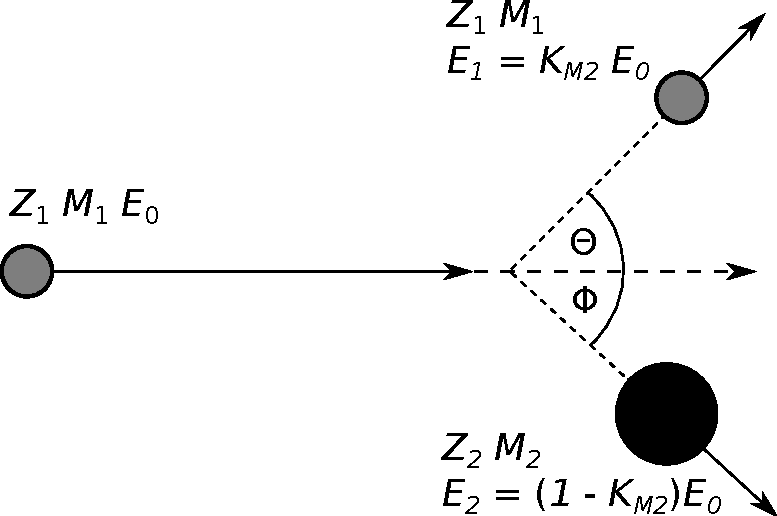
\includegraphics[width=80mm]{rutherford.pdf}
  \caption{Geometrie pružného rozptylu částice s~atomovým číslem $Z_1$, hmotností $M_1$ a~energií $E_0$ na atomovém jádru ($Z_2$, $M_2$)}
  \label{rutherford}
\end{figure}

Některé z~dopadajících částic se rozptýlí na atomech obsažených v látce a~jsou analyzovány spektrometrem, který určí jejich energii. Při pružném rozptylu předává částice část své kinetické energie atomu, ale celková kinetická energie soustavy částice--atom se zachovává. Energie předaná atomu závisí pouze na hmotnostech částice $M_1$, atomu $M_2$ a~na úhlu rozptylu $\Theta$. z~jednoduché kinematické úvahy vyplývají pro energie rozptýlené částice $E_1$ a~atomu $E_2$ po srážce vztahy
%
\begin{equation}
E_1 = K_{M_2} E_0 \mathrm{,}
\end{equation}
\begin{equation}
E_2 = (1 - K_{M_2}) E_0 \mathrm{,}
\end{equation}  
%
kde $K_{M_2}$ je tzv. kinematický faktor a~je dán vztahem
\begin{equation}
K_{M_2} = \left[ \frac{\sqrt{M_2^2 - M_1^2\sin^2\Theta} + M_1 \cos\Theta}{M_1 + M_2} \right]^2 \mathrm{,}
\end{equation}
schéma srážky je na obrázku \ref{rutherford}.

Další, z~hlediska analytického využití metody RBS významnou veličinou je účinný průřez pružného rozptylu, který spojuje počet rozptýlených částic s~počtem atomů v látce. Ve standardním uspořádání metody RBS může být pružný rozptyl popsán s~dostatečnou přesností jako rozptyl částice v centrálním elektrostatickém poli nestíněného atomového jádra. V takovém případě je diferenciální účinný průřez rozptylu pod laboratorním úhlem $\Theta$ dán vztahem
\begin{equation}
\frac{\mathrm{d}\sigma_\mathrm{R}}{\mathrm{d}\Omega} = 
\left( \frac{Z_1 Z_2 e^2}{2 E_0} \right)^2
 \frac{ \left[ \sqrt{M_2^2 - M_1^2\sin^2\Theta} + M_2 \cos\Theta \right]^2 }{M_2 \sin^4 \Theta \sqrt{M_2^2 - M_1^2\sin^2\Theta}}  \mathrm{,}
\end{equation}
kde $e$ je elementární náboj. Tento vztah pro účinný průřez nicméně platí pouze v případě, kdy částice pronikne až do blízkosti jádra rozptylujícího atomu a~při rozptylu lze zanedbat stínící efekt elektronového obalu. Při analýzách pomocí těžších částic a~při nižších energiích může elektronové stínění hrát významnější roli. Pro vysoké energie částic a~pro částice s~nižším atomovým číslem naopak musíme vzít do úvahy interakce částice s~atomovým jádrem prostřednictvím jaderných sil.

Podrobnější analýzou měřených spekter pak lze kromě povrchových koncentrací určit i~hloubkové koncentrační profily měřených vrstev. 


\subsubsection{Detekce vyražených atomů - metoda ERDA}
\begin{figure}[bthp]
  \centering
  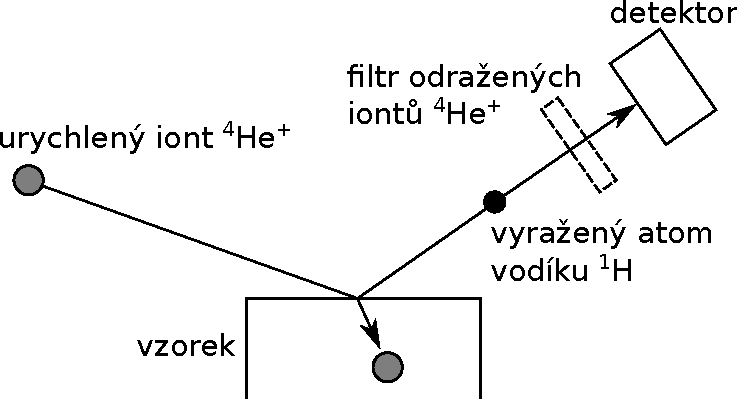
\includegraphics[width=90mm]{ERDA.pdf}
  \caption{Schéma metody ERDA pro měření vodíku}
  \label{ERDA}
\end{figure}

Detekce lehkých prvků metodou RBS je obtížná vzhledem k nízkým účinným průřezům elastického rozptylu a~často i~proto, že příslušný analytický signál leží na vysokém pozadí vzniklým rozptylem částic na těžších prvcích. 
V případě, kdy částice mají větší hmotnost než atomy látky, k jejich rozptylu do velkých úhlů nedochází vůbec a~analýza standardním postupem není možná. V takovém případě lze s~výhodou použít metodu ERDA, která je založena na detekci a~energetické analýze atomů vyražených dopadajícími částicemi z~ana\-ly\-zované látky. 
Metoda ERDA je tedy postupem inverzním k běžné metodě RBS. Princip detekce atomů vodíku v nejjednodušší variantě metody ERDA je znázorněn na obrázku \ref{ERDA}. Na vzorek dopadají monoenergetické částice $\alpha$ pod malým úhlem, zpravidla menším než 15$^\circ$ vzhledem k povrchu. 
Při jejich elastickém rozptylu dochází k vyražení lehčích atomů vodíku ze vzorku. Tyto vyražené atomy pak mohou být registrovány a~energeticky analyzovány běžným polovodičovým detektorem. 
Atomy vyražené z~vrstev pod povrchem vzorku jsou registrovány s~energií sníženou o energetické ztráty dopadajících částic a~atomů vyražených z~materiálu vzorku. Z~tvaru energetického spektra lze pak zjistit hloubkový koncentrační profil vodíku. 

\cleardoublepage


\end{document}
